\documentclass[../report.tex]{subfiles}

\begin{document}
\noindent Xét dãy số $x_i$ có $N$ phần tử, 
$i = \overline{0, N - 1}$,
$N = 2^p$, ta có: 
\begin{align*}
    X_u &= \mathcal{F}[x_i]_u = \sum_{i = 0}^{N - 1} x_i 
    e^{-j\frac{2\pi i u}{N}} \\
    &= \sum_{i = 0}^{\frac{N}{2} - 1} 
    x_{2i} e^{-j\frac{2\pi 2 i u}{N}}
    + \sum_{i = 0}^{\frac{N}{2} - 1} x_{2i + 1} 
    e^{-j\frac{2\pi (2i + 1) u}{N}} \\
    &= \sum_{i = 0}^{\frac{N}{2} - 1} 
    x_{2i} e^{-j\frac{2\pi i u}{N/2}}
    + e^{-j\frac{2\pi u}{N}} 
    \sum_{i = 0}^{\frac{N}{2} - 1} x_{2i+ 1} 
    e^{-j\frac{2\pi i u}{N / 2}}
\end{align*}

\noindent Đặt: $a_i$ là dãy các số có chỉ số chẵn lấy ra từ $x_i$. \\
\hspace*{22pt} $b_i$ là dãy các số có chỉ số lẻ lấy ra từ $x_i$.

\noindent Ta được: 
\begin{align*}
    \sum_{i = 0}^{\frac{N}{2} - 1} x_{2i} e^{-j\frac{2\pi i u}{N/2}}
    &= \sum_{i = 0}^{\frac{N}{2} - 1} a_i e^{-j\frac{2\pi i u}{N/2}} \\
    &= \mathcal{F}[a_i]_u 
    \quad\quad\left(\textrm{Có }\frac{N}{2}\textrm{ phần tử}\right) \\
    \sum_{i = 0}^{\frac{N}{2} - 1} x_{2i + 1} e^{-j\frac{2\pi i u}{N/2}}
    &= \sum_{i = 0}^{\frac{N}{2} - 1} b_i e^{-j\frac{2\pi i u}{N/2}} \\
    &= \mathcal{F}[b_i]_u
    \quad\quad\left(\textrm{Có }\frac{N}{2}\textrm{ phần tử}\right)
\end{align*}
Nhưng lại có: $u = \overline{0, N - 1}$ \\[5mm]

\noindent Tuy nhiên, ta có thể thấy:
\begin{align*}
    e^{-j\frac{2\pi i u}{N/2}} 
    &= e^{-j\frac{2\pi i u}{N/2} + j 2\pi i}  \\
    &= e^{-j\frac{2\pi i (u - N/2)}{N/2}}
\end{align*}
Tuần hoàn với chu kì $\frac{N}{2}$ \\
Nên ta chỉ cần tính $\frac{N}{2}$ giá trị $u$ cho 
$\mathcal{F}[a_i]_u$ và $\mathcal{F}[b_i]_u$ là đủ. Đây cũng
chính là mấu chốt làm cho thuật toán FFT có thể thực hiện được với 
thời gian $\mathcal{O}(N \log N)$. \\[5mm]

\noindent Từ đó: \\
Nếu xét với $u = \overline{0, \frac{N}{2} - 1}$
\begin{align*}
    \mathcal{F}[x_i]_u &= \mathcal{F}[a_i]_u 
    + e^{-j\frac{2\pi u}{N}} \mathcal{F}[b_i]_u \\
    \mathcal{F}[x_i]_{u + N/2} &= \mathcal{F}[a_i]_u 
    + e^{-j\frac{2\pi (u + N/2)}{N}} \mathcal{F}[b_i]_u \\
    &= \mathcal{F}[a_i]_u 
    - e^{-j\frac{2\pi u}{N}} \mathcal{F}[b_i]_u
\end{align*}\\[5mm]

\noindent Thời gian tính toán:  \\
Gọi $T(n)$ là thời gian tính cho giải thuật này, áp dụng
định lý thợ, ta được: 
\begin{align*}
    &T\left(n\right) = 2 T\left(\frac{n}{2}\right) 
    + \Theta \left(n\right) \\
    &\Rightarrow T(n) = \Theta \left( n \log n\right)
\end{align*}

\noindent Ta có thể sử dụng đệ quy để implement thuật toán FFT. 
Tuy nhiên cách implement đó là không hiệu quả, trong các bài toán 
nhân nhanh đa thức và trong thực tế thì người ta thường sử dụng 
thuật toán như sau: 
\begin{itemize}
\item Hoán vị các phần tử sử dụng đảo bit 
giá trị nhị phân các chỉ số trong mảng. Như được 
biểu diễn bằng hình sau: 
\begin{figure}[H]
\centering
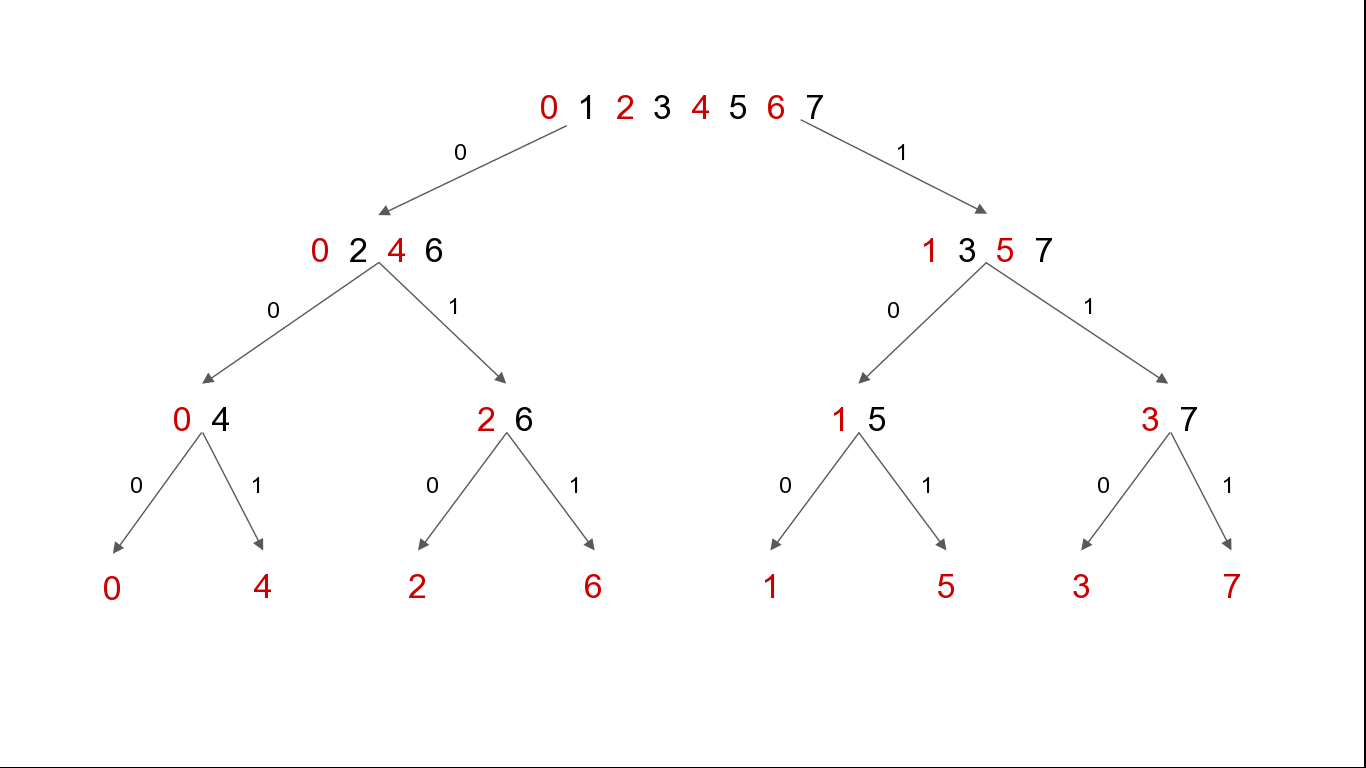
\includegraphics[width=\textwidth]{figures/swap.png}
\end{figure}
\item Thực hiện vòng lặp tính các DFT từ 
$n = 2$ và tăng dần $\times 2$
mỗi vòng lặp, như hình dưới đây: 
\begin{figure}[H]
\centering
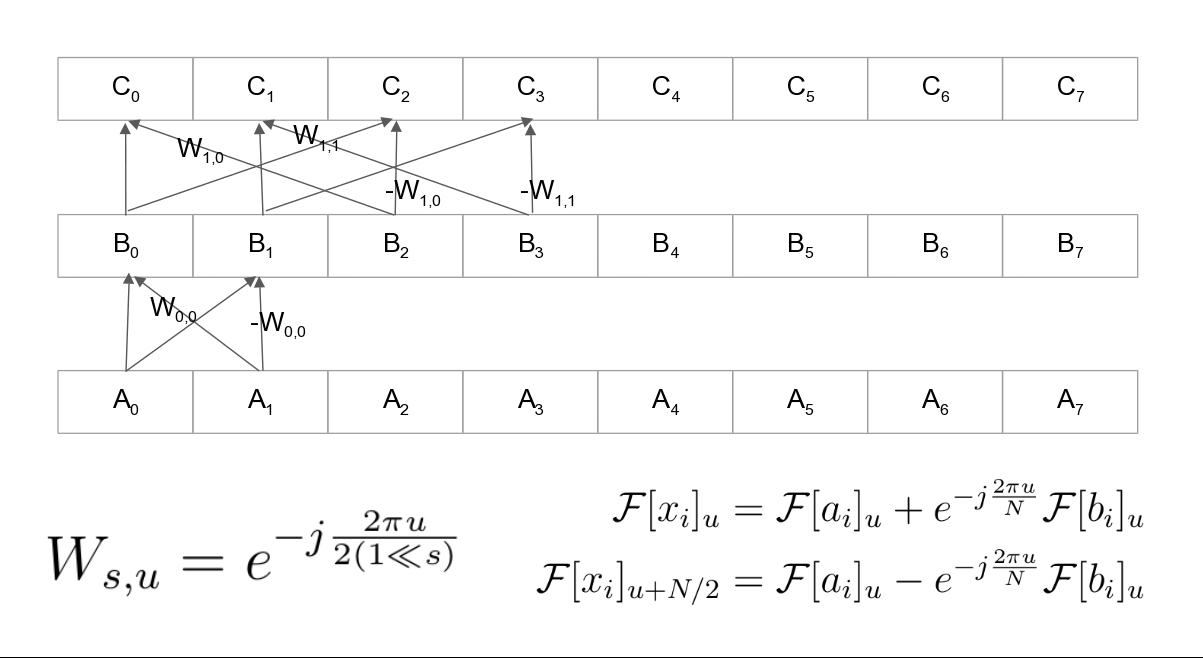
\includegraphics[width=\textwidth]{figures/fft.png}
\end{figure}

\end{itemize}
Code của thuật toán FFT: 
\begin{lstlisting}
std::bitset<64> reverse(std::bitset<64> set, ll bit_count) {
    for (ll i = 0; i < bit_count / 2; i++) {
        bool tmp = set[i];
        set[i] = set[bit_count - 1 - i];
        set[bit_count - 1 - i] = tmp;
    }
    return set;
}

void init_T(ll bit_count) {
    ll N = 1 << bit_count;
    for (ll i = 0; i < N; i++)
        T[i] = reverse(i, bit_count).to_ullong();
}

void fft(cp *A, ll bit_count, bool inverse = false) {
    static cp W[FFT_MAX / 2];

    ll N = 1 << bit_count;

    for (ll i = 0; i < N; i++) {
        ll j = T[i];
        if (i < j) 
            std::swap(A[i], A[j]);
    }

    for (ll step = 1; step < N; step <<= 1) {
        double angle = -PI / step;
        if (inverse)
            angle = -angle;

        cp w(1, 0), wn(std::cos(angle), std::sin(angle));
        for (ll i = 0; i < step; i++) {
            W[i] = w;
            w *= wn;
        }

        for (ll start_even = 0; start_even < N; start_even += step * 2) {
            auto start_odd = start_even + step;
            for (ll i = 0; i < step; i++) {
                cp U = A[start_even + i];
                cp V = W[i] * A[start_odd + i]; 
                A[start_even + i] = U + V;
                A[start_odd + i] = U - V;
            }
        }
    }

    if (inverse) {
        for (ll i = 0; i < N; i++)
            A[i] /= N;
    }
}
\end{lstlisting}
Trong đó init\_T dùng để khởi tạo mảng chuyển vị T. step là biến biểu 
thị rằng các giá trị FFT với kích thước step đã được tính. Biến inverse = true khi mà ta muốn tính FFT ngược. 

\end{document}
